\chapter{Wyniki eksperymentu}
\label{c5}

Dany rozdział zawiera wyniki z przeprowadzonych badań oraz wnioski. Każda aplikacja, która została napisana została przestawiona i opisana z różnych perespektyw. Na końcu rozdziału zostały przedstawione wady i zalety obu podejść.

\section{Stworzone aplikacje}

Aplikacje zostały najpierw stworzone w App Inventorze, a następnie zostały przepisane na język Java.

\subsection{Sortowanie}

Aplikacja polega na wygenerowaniu listy losowych elementów, a następnie posortowaniu jej. Do sortowania został użyty prosty algorytm sortowania przez wybieranie \english{Selection Sort}.

\begin{figure}[th] 
\centering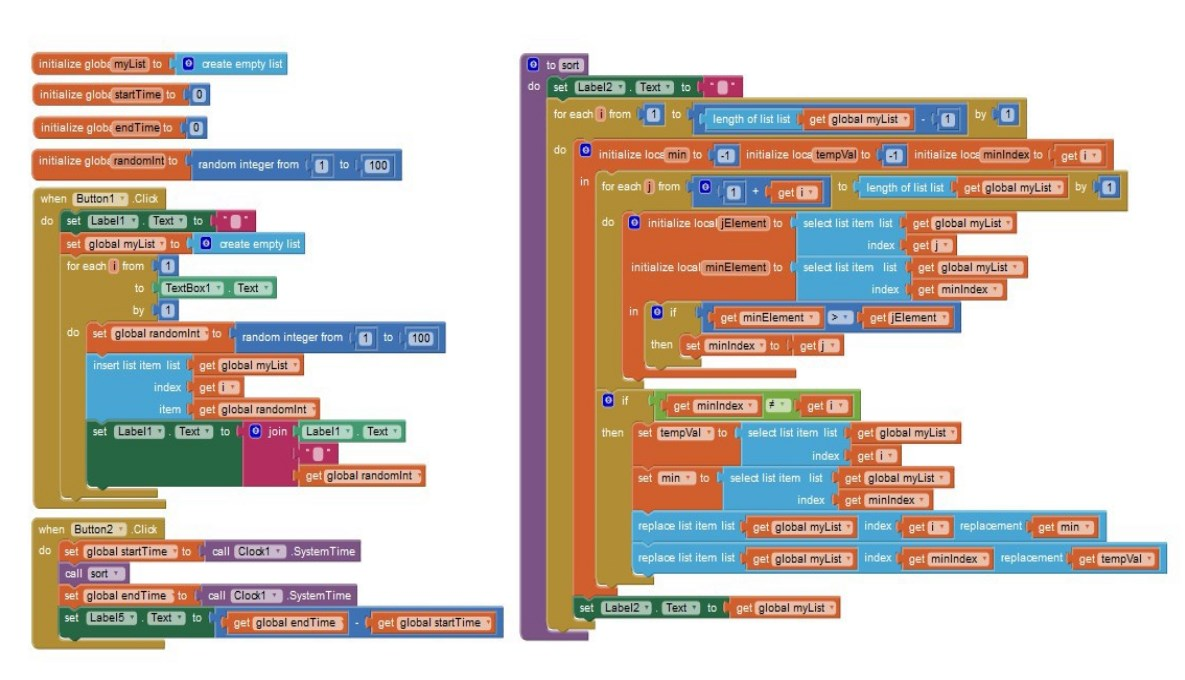
\includegraphics[width=15cm]{figures/apps/sort}
\caption{Aplikacja sortująca - App Inventor}
\end{figure}

Na powyższym rysunku widać bloki potrzebne do stowrzenia aplikacji w App Inventorze. Bez głębszej analizy zrozumienie działania bloków, może okazać się kłopotliwe. Jest to prosty algorytm, a napisanie go za pomocą dostępnych bloków okazało się skomplikowane. Można sobie łatwo wyobrazić, że napisanie bardziej skomplikowanego algorytmu byłoby bardzo nieczytelne. Ilość użytych bloków zdecydowanieby wzrosła, dodatkowo utrzymanie takiej aplikacji niesie za sobą wysokie koszty wprowadzenia nowych osób do jej rozwijania.

Sortowanie napisanie w javie jest zrozumiałe dla każdego programisty. Do sortowania została użyta lista, jako odpowiednik listy w App Inventorze, nie ma tam dostępnych tablic.


\begin{lstlisting}
 void sort(List<Integer> list){
        for(int i =0;i<list.size()-1;i++){
            int index = i;
            for(int j=i+1;j<list.size();j++){
                if(list.get(j) < list.get(index) ){
                    index = j;
                }
            }
            if(index != i){
                int tmp = list.get(i);
                list.set(i,list.get(index));
                list.set(index,tmp);
            }
        }
    }
\end{lstlisting}

W algorytmach bardzo ważna jest wydajność. Oba algorytmy działają w ten sam sposób, jednak wydajność sortowania listy napisanej w Javie jest zdecydowanie wyższa. Można to zaobserwować na poniższym wykresie. Przesortowanie bardzo małej liczby elementów zajmuje App Inventorowi bardzo dużo czasu. Przy 25 elementach czas sortowania przekroczył 1 sekundę. Jest to bardzo słaby wynik w porównaniu do sortowania napisanego w Javie. Średnio czas sortowania był 2 tysiące razy mniejszy! Na danym wykresie została zastosowana skala logarytmiczna, aby zobaczyć różnicę.

\begin{figure}[htbp]
\centering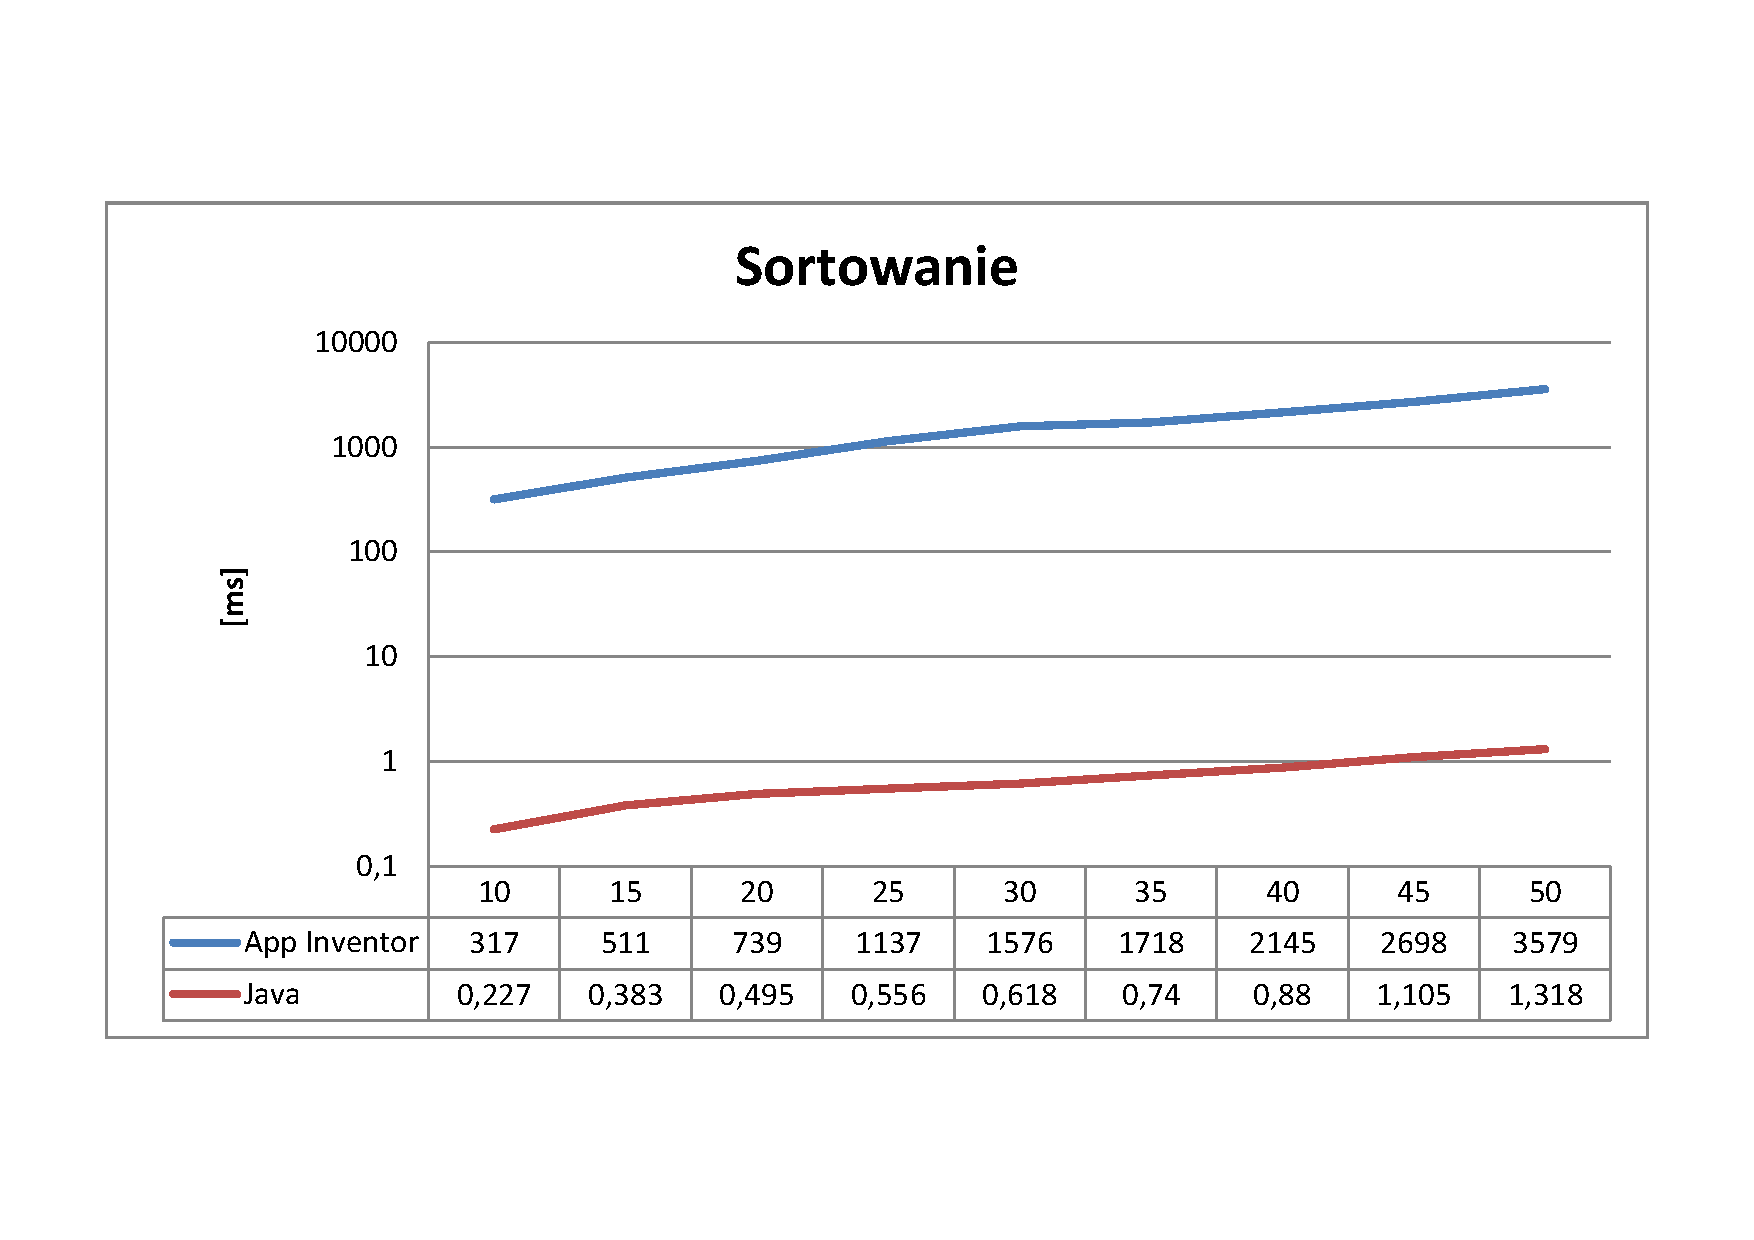
\includegraphics[width=10cm]{figures/apps/sortChart}
\caption{Wykres przedstawiający czas sortowania}
\end{figure}

Napisanie tej aplikacji w Javie nie było żadnym problemem. Bardzo łatwo było zdebugować kod i sprawdzić jego poprawność. Stworzenie tej samej aplikacji w App Inventorze nie było trywialne.


\subsection{Akcelerometr}

Kolejną aplikacją jest wykorzystująca akcelerometr. Odczytuje ona dane z akcelerometru, a następnie wyświetla je na ekran telefonu, z zadaną częstotliwością. Na poniższym wykresie przedstawione jest zużycie procesora dla różnych wartości próbkowania. Można zauważyć, że zużycie procesora dla aplikacji napisanej w Javie jest prawie stałe. Dzieje się tak dlatego że ustawianie częstotliwości próbkowania jest to tylko wskazówką dla systemu. Zdarzenia mogą być odbierane szybciej lub wolniej niż zadana częstotliwość. Zazwyczaj są odbierane szybciej. W tym przypadku są odbierane szybciej i zmiana częstotliwości na mniejszą, tak naprawdę nic tutaj nie zmienia, ponieważ zdarzenia dalej będą odbierane szybciej. Zużycie procesora prawdopodobnie będzie dalej stałe, gdy będziemy zmniejszać częstotliwość.\cite{doc:android}

\begin{figure}[H]
\centering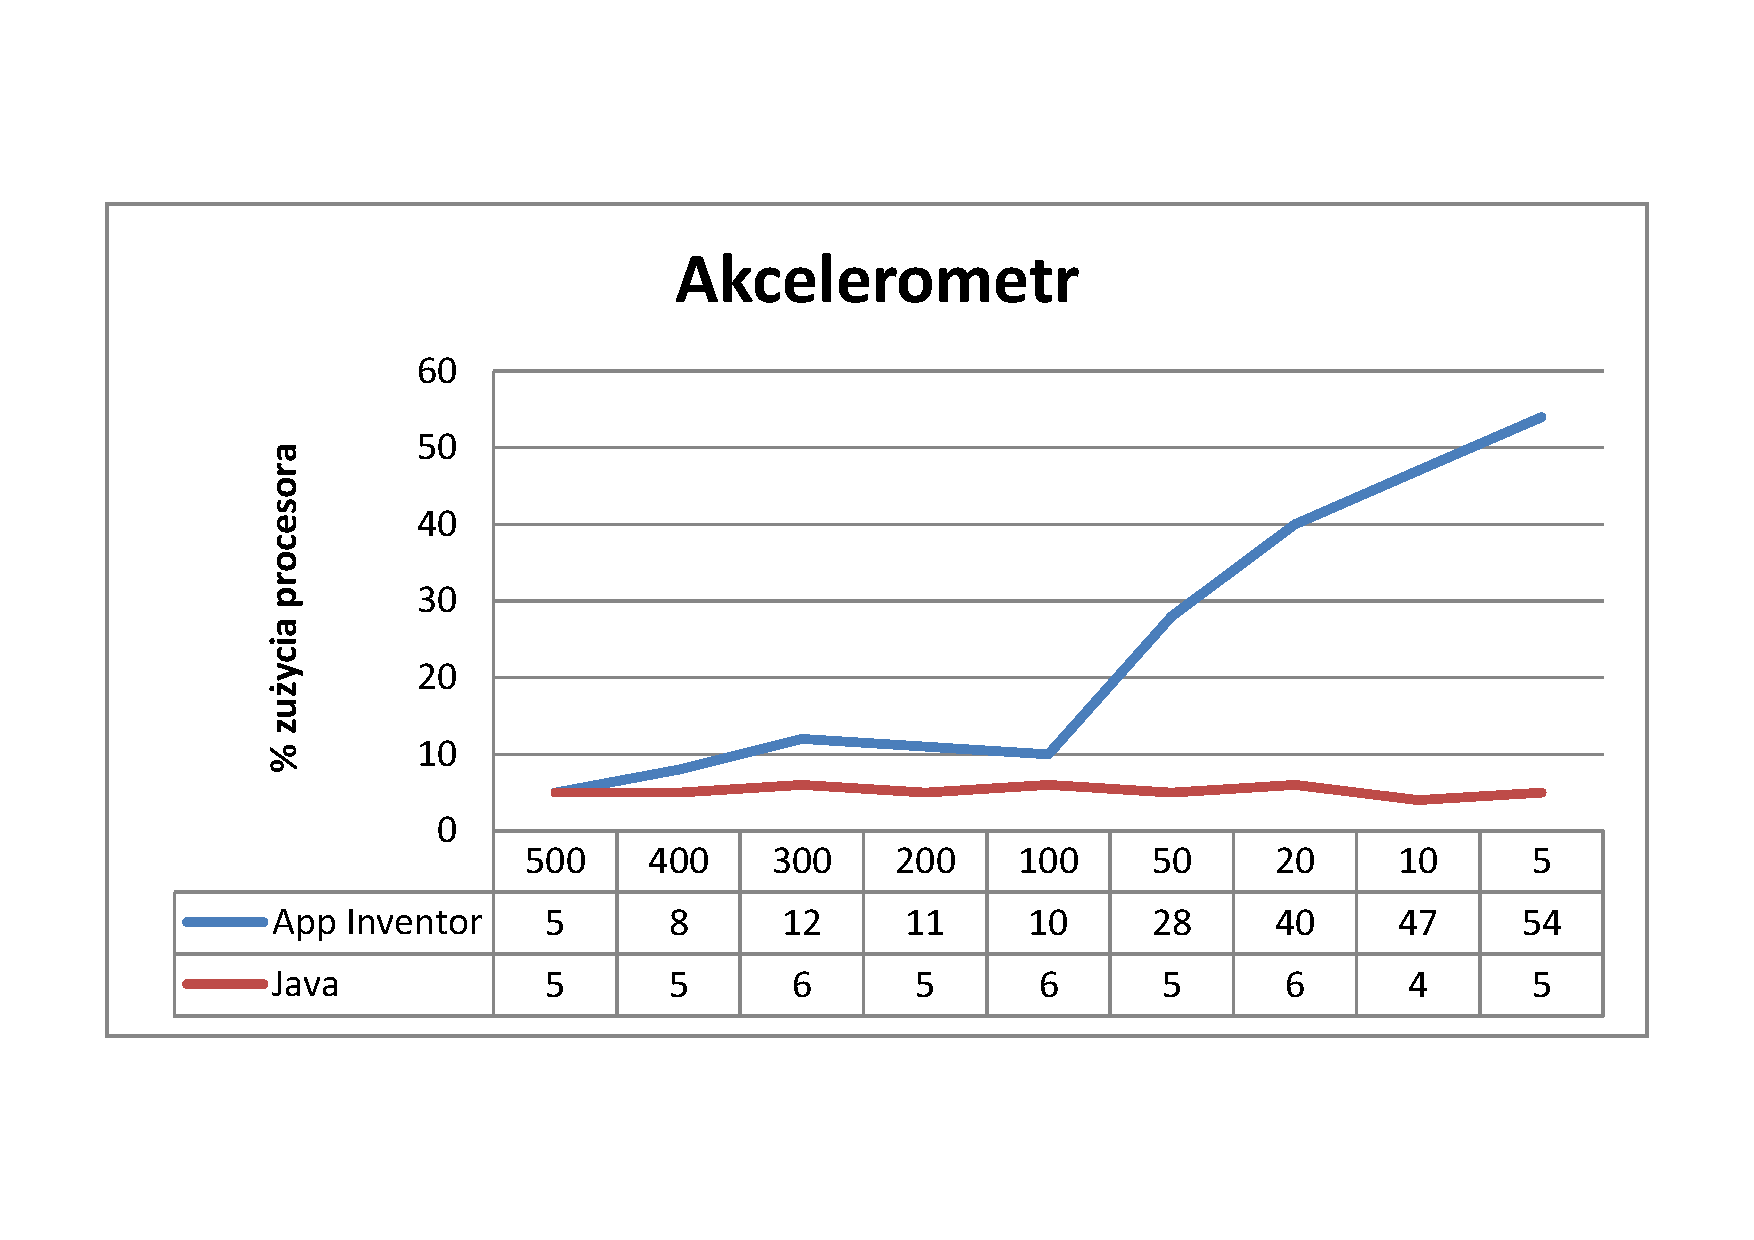
\includegraphics[width=10cm]{figures/apps/accelerometerChart}
\caption{Wykres przedstawiający zużycie procesora}
\end{figure}

W AppInventorze nie można zadać bezpośrednio akcelerometrowi częstotliwości próbkowania. Aby to obejść, trzeba dodać nowy komponent Clock, który ma możliwość uruchamiania, co zadany czas. Można podejżewać, że wydajność akcelerometru jest niezmienna i częstotliwość próbkowania jest stała. Wyraźny spadek wydajności jest przez to, że musimy wywoływać metody w bardzo krótkich odstępach czasu i to, że one dodatkowo odczytują wartość sensora, nie wpływa znacząco na zużycie procesora.


\subsection{Fibonacci}

Następną stworzoną aplikacją jest aplikacja wyliczająca kolejny element ciągu Fibonnaciego. Testuje ona wydajność App Inventora. Złożoność takiego algorytmu to $O(2^n)$, czyli czas wykonywania będzie rósł bardzo szybko. Dodatkowo, kod jest napisany tak, aby metody wykonywały się rekurencyjnie, jednak aplikacja nie jest w stanie przetestować wielkości stosu. Dla bardzo małych liczb czas wykonywania się algorytmu jest bardzo wysoki.

\begin{figure}[H]
\centering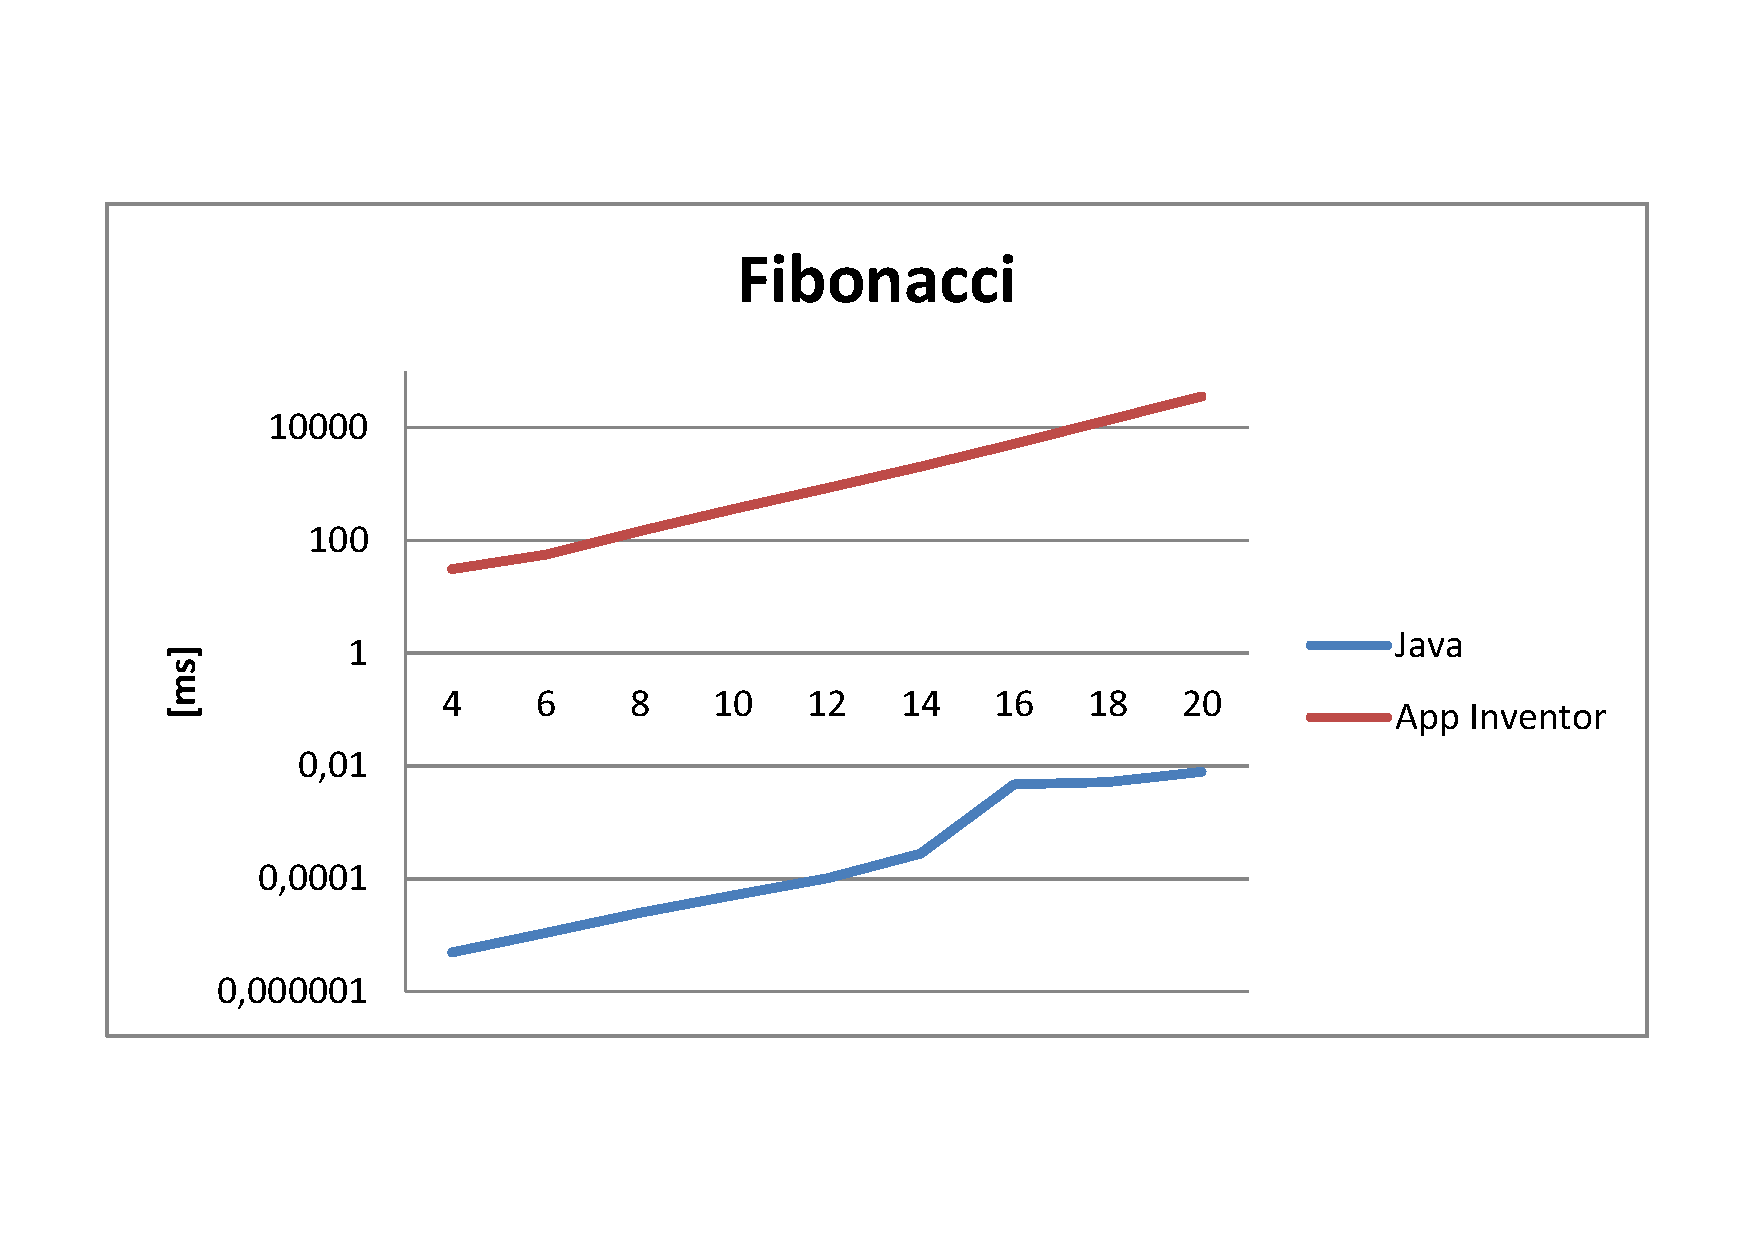
\includegraphics[width=10cm]{figures/apps/fibonacciChart}
\caption{Wykres przedstawiający czas obliczenia n-tego elementu z ciągu Fibonacciego}
\end{figure}

Osiągnięty rezultat wydajności nie jest zaskakujący po otrzymaniu wyników z poprzednich programów. Czas obliczenia już początkowych elementów ciągu Fibonnaciego jest bardzo duży. Przy liczeniu 20 elementu aplikacja napisana w App Inventorze potrzebuje ponad pół minuty, podczas gdy, aplikacja napisana w Javie potrzebuje na to około jedną setną sekundy.


\subsection{Silnia}

Następny program oblicza silnię danego elementu. Istnieje możliwość wyboru, iteracyjna lub rekursyjna wersja. Aby zaprezentować oba podejścia na jednym wykresie, została użyta skala logarytmiczna.

\begin{figure}[H]
\centering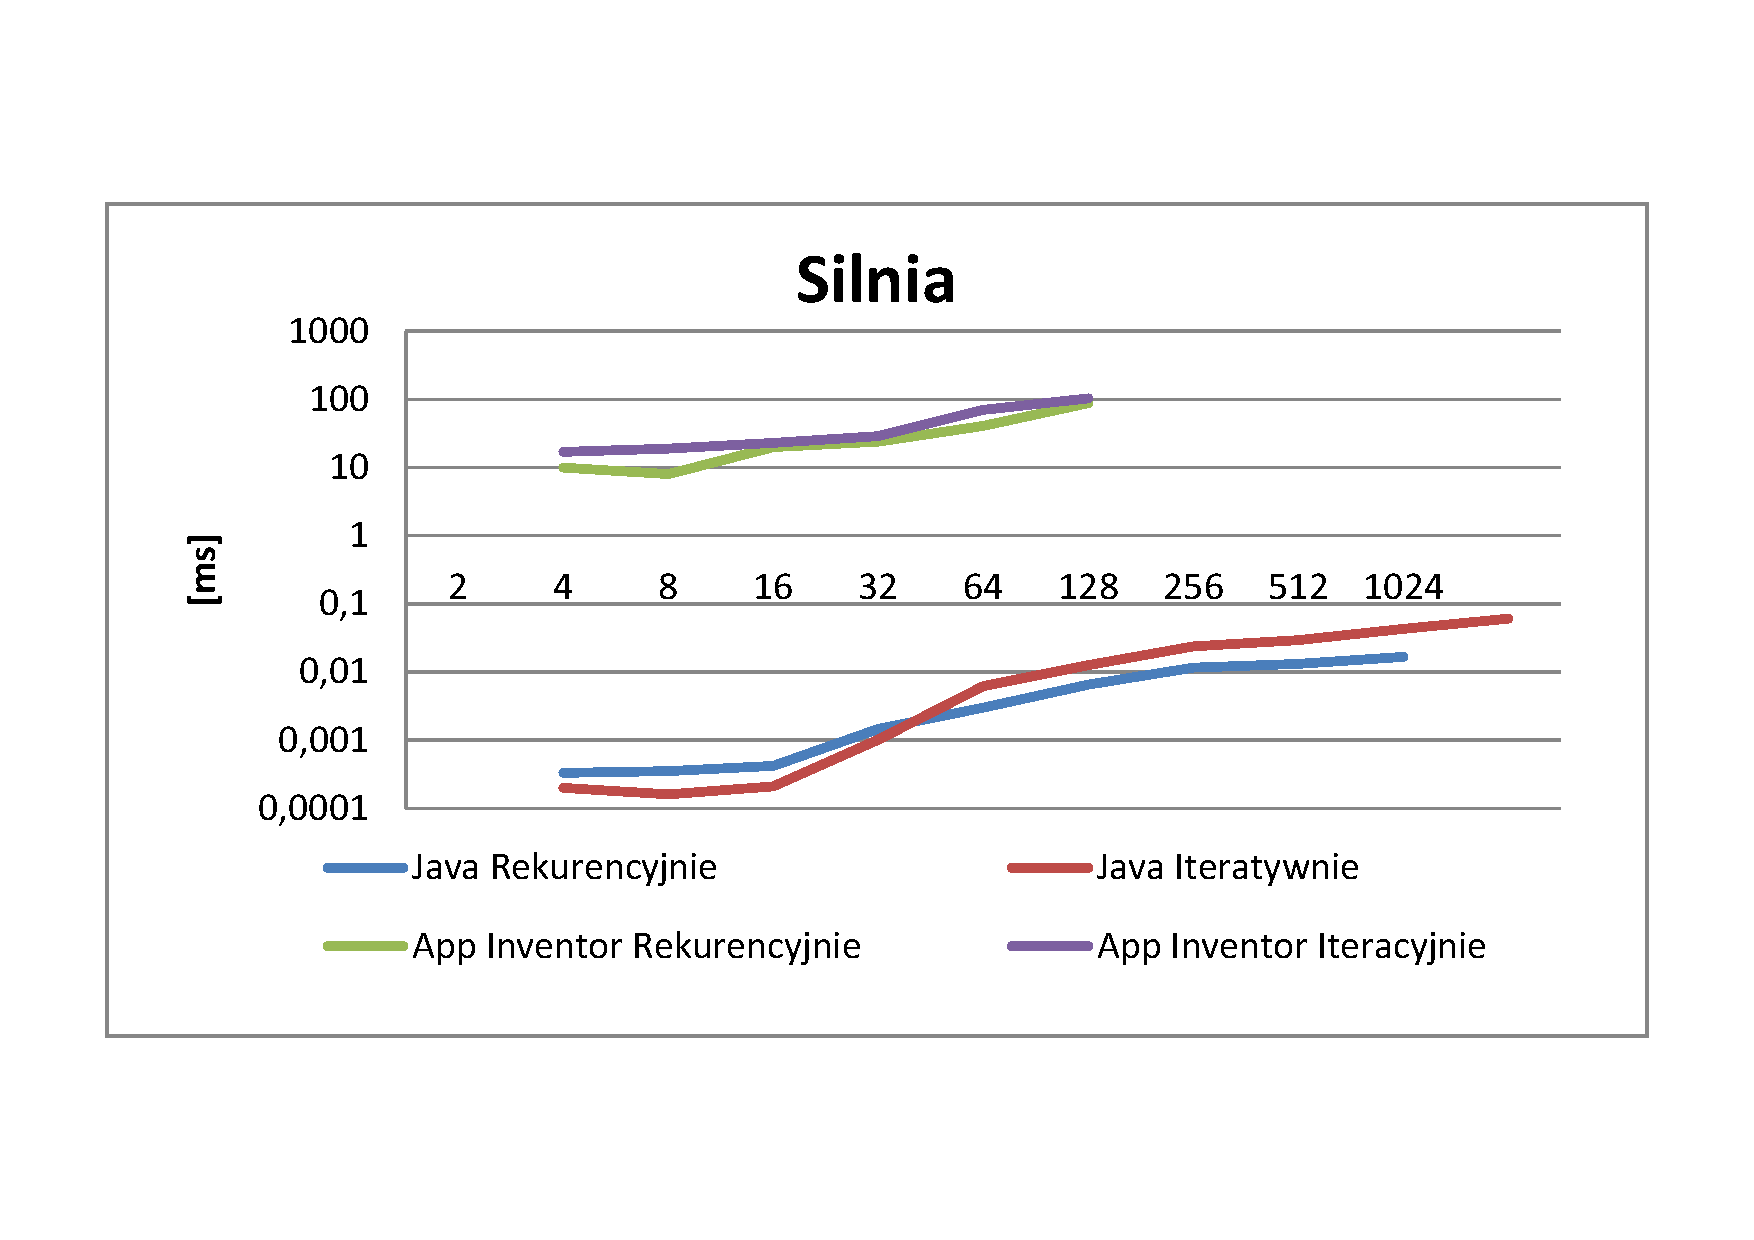
\includegraphics[width=10cm]{figures/apps/factorialChart}
\caption{Wykres przedstawiający czas obliczenia silni danego elementu}
\end{figure}

Na powyższym wykresie można zaobserować wiele istotnych elementów. Aplikacja napisana w języku Java nie miała żadnych problemów w podejściu iteracyjnym. Zakres liczb nie został przekroczony, ze względu na możliwość wyboru typu danych. Potrzebna była tutaj klasa dla wielkich liczb całkowitych, dlatego został użyty typ BigInteger. Podczas użycia wersji rekurencyjnej, przy około liczeniu silni dla około 700, program rzuca wyjątek przepełnienia stosu (\english{Stack overflow}).

Ciekawa sytuacja występuje dla aplikacji napisanej w App Inventorze. Program rzuca wyjątek podczas działania programu (\english{Runtime error}). Niestety, nie wiadomo co to za błąd, ponieważ w logach wiadomość o błędzie jest niedostępna. Wiadomość, którą otrzymujemy w logach wygląda następująco:

\begin{lstlisting}
E/com.google.appinventor.components.runtime.util.RuntimeErrorAlert:
No error message available
\end{lstlisting}

Można się jedynie domyślać, że jest to błąd przepełnienia stosu lub przekroczenia zakresu liczb.

\subsection{Database}

Aplikacja stworzona aby sprawdzić szybkość działania bazy danych oferowanej przez App Inventora. Został tutaj wykorzystany komponent TinyDB. Odpowiada on klasie Javy SharedPreferences, czyli jest to baza danych typu klucz/wartość. Aby odczytać dane z pamięci trzeba znać klucz do tych danych. Jest to bardzo łatwe w przypadku małych ilości danych, jednak trudno jest przechowywać większy struktury, ze względu na potrzebę znania klucza dla każdego wiersza. Duże ilości danych powinny być przechowywane w bazie danych SQLite, ponieważ organizacja danych i zarządzanie nimi jest wydajniejsze. Aby otrzymać część danych z bazy, trzeba posłużyć się językiem zapytań SQL. Daje to możliwość wyszukiwania interesujących nas danych. Z drugiej strony zarządzanie i przeszukiwanie dużych zbiorów danych wpływa na wydajność, więc czytanie danych z bazy danych może być wolniejsze niż czytanie danych z SharedPreferences.

\begin{figure}[H]
\centering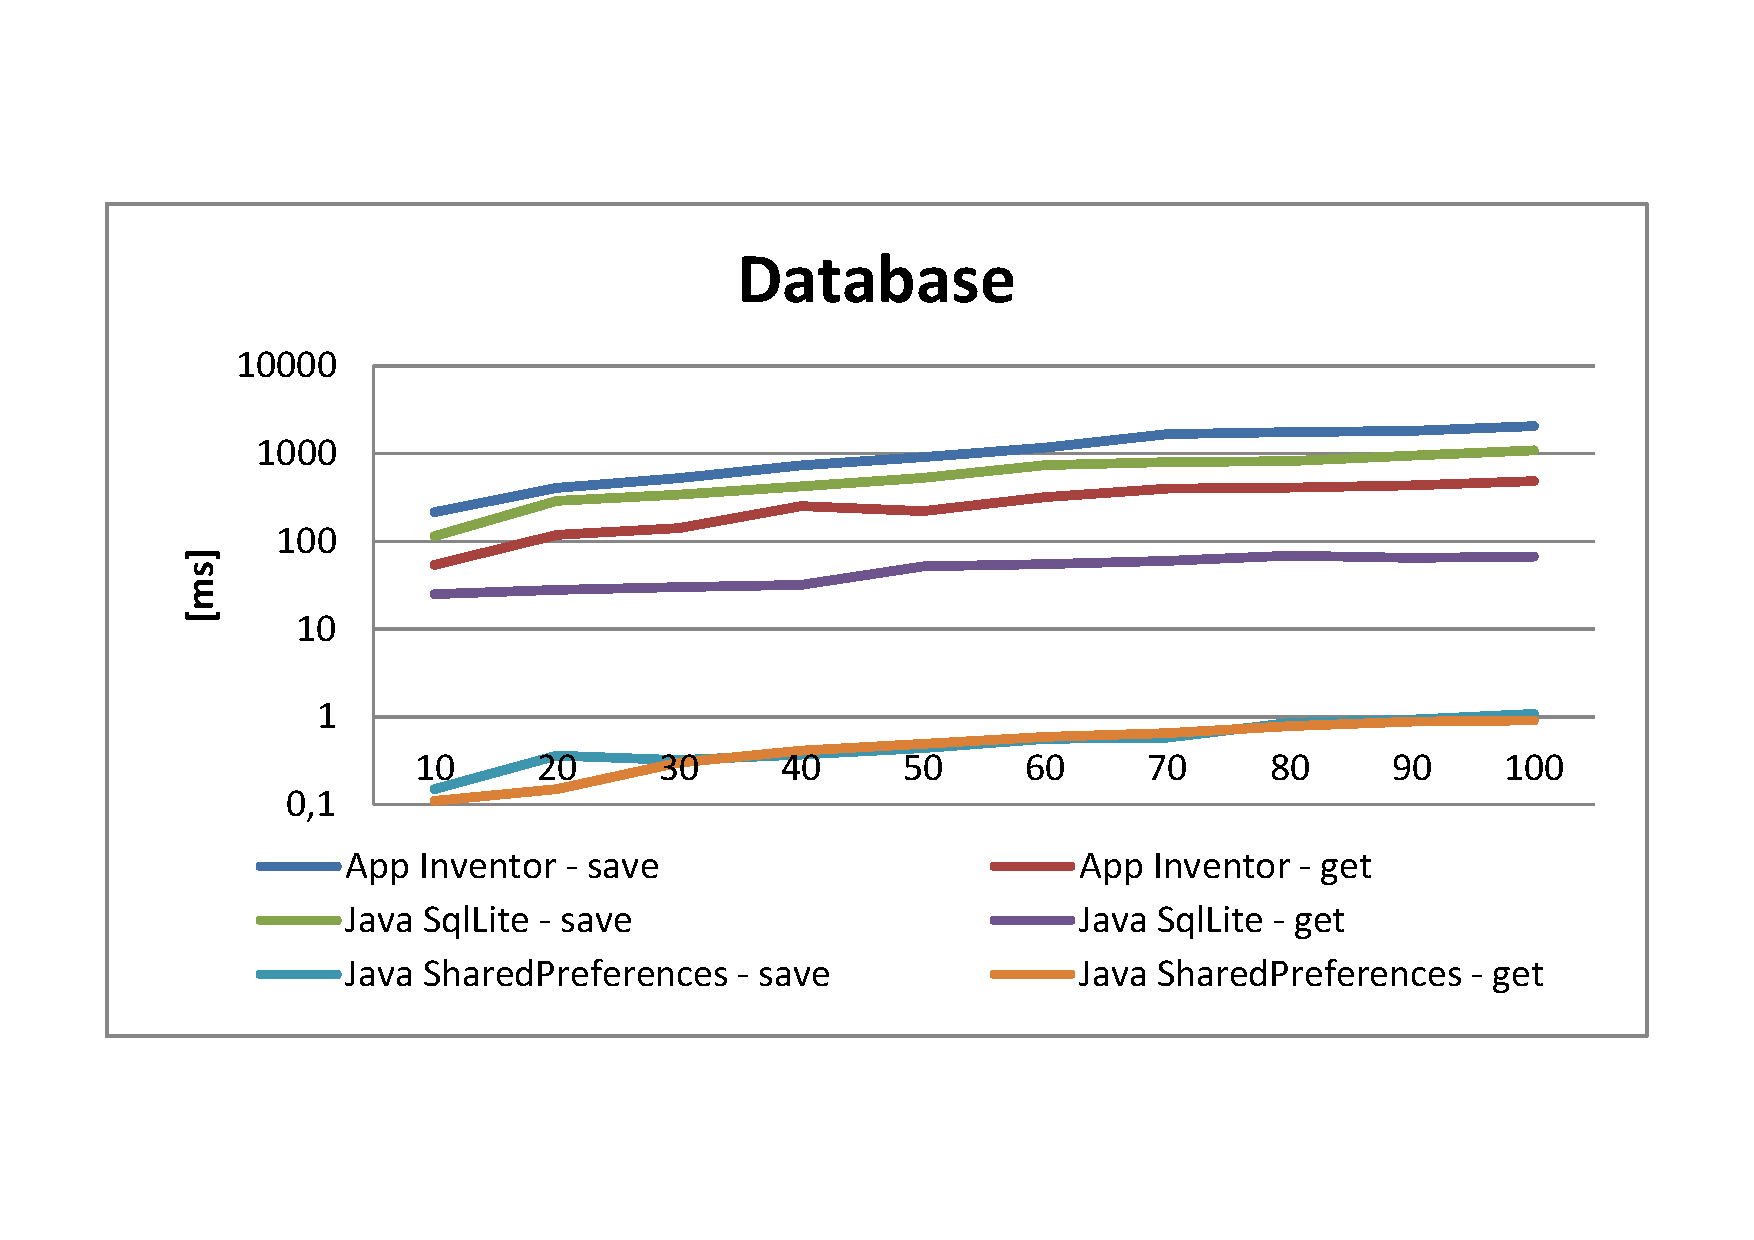
\includegraphics[width=10cm]{figures/apps/databaseChart}
\caption{Wykres przedstawiający czas potrzebny na zapis/odczyt n-elementów}
\end{figure}

Na powyższym wykresie można zauważyć przewagę wydajności aplikacji napisanej w Javie. App Inventor uzyskał podobny rezultat wydajności, jak aplikacja napisana w Javie, która używa bazy danych SQLite. Jak wspomniano wcześniej odczyt/zapis danych z bazy SQLlite powinien być wolniejszy niż korzystanie z SharedPreferences. SQLite uzykuje tutaj lepszy rezultat TinyDB - odpowiednik SharedPreferences. Można łatwo wyciągnąć wniosek, że wydajność TinyDB jest bardzo niska. Jeżeli porównamy TinyDB i SharedPreferences przewaga aplikacji napisanej w Javie jest ogromna.


\subsection{Animacja}

Aplikacja testuje możliwości animacyjne App Inventora. Wiadomo że komponenty potrzebne są dostępne, jednak nie wiadomo, czy wydajność pozwoli na płynną animację. Mimo że tworzenie animacji może wydawać się trudne, za pomocą App Inventora stworzenie animacji odbywa się tylko w kilku krokach. Największym problemem było znalezienie odpowiednich klatek, gdzie ostatnia wygląda tak samo jak pierwsza, aby była możliwość zapętlenia.


\begin{figure}[H]
\centering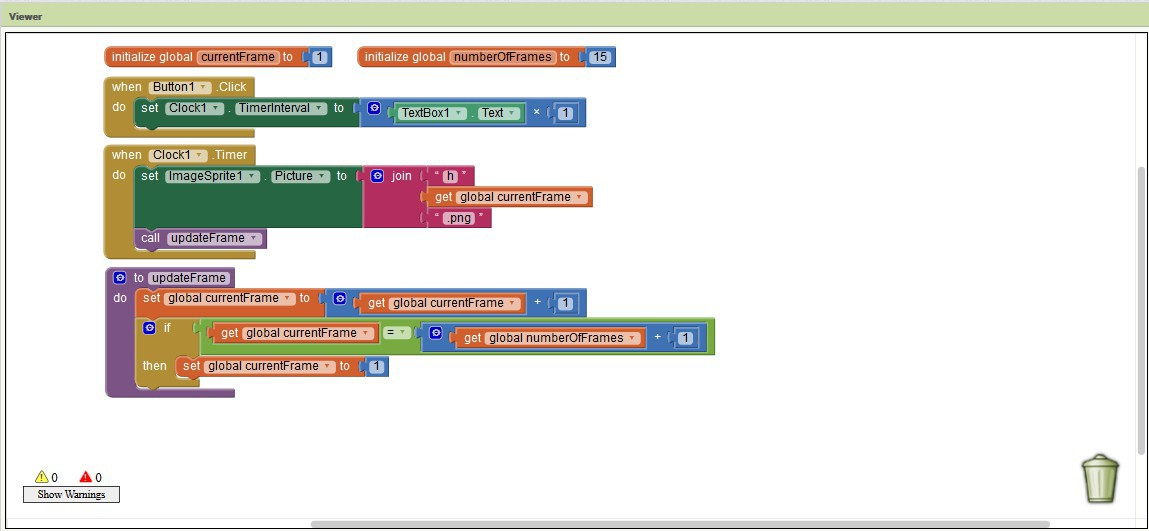
\includegraphics[width=15cm]{figures/apps/ai_animation}
\caption{Bloki potrzebne do stworzenia aplikacji}
\end{figure}

Na głównym ekranie aplikacji stworzone jest płótno oraz jeden obrazek, który podmieniamy co zadany interwał czasu. Ostatecznym rezulatatem jest płynna animacja. Dopiero przy bardzo niskim interwale czasowym (szybkiej zmianie klatek), można być odczyć przycinanie się ekranu.


\subsection{Kolizja elementów}

Aplikacja sprawdzająca możliwość detekcji kolzji poruszających się elementów. Na płótnie zostało umieszczone kilka elementów. Elementy w kolorze czarnym poruszają się po płótnie i kiedy dotrą do ściany odbijają się od niej. Element o kolorze niebieskim jest sterowanym za pomocą akcelerometru. Pochylając telefon przesuwamy element po płaszczyźnie.

\begin{figure}[H]
\centering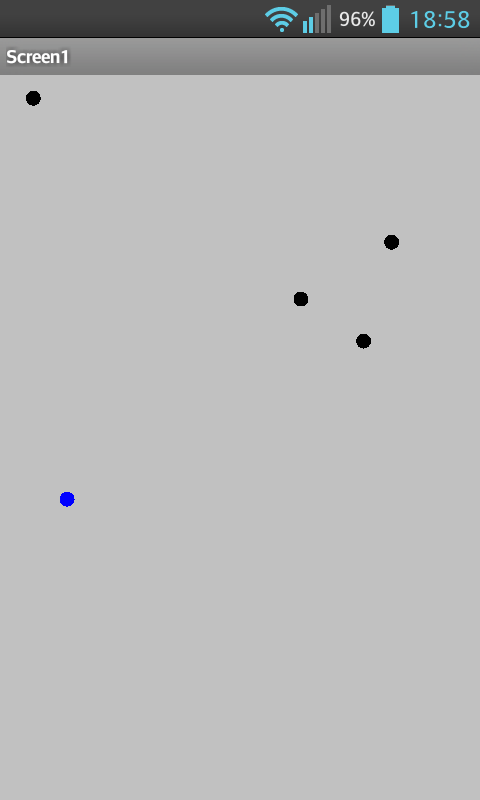
\includegraphics[width=5cm]{figures/apps/ai_collision}
\caption{Wygląd aplikacji testującec kolizje}
\end{figure}

Aplikacja działa płynnie, dla takiej ilości elementów. Wadą, którą można tutaj zauważyć, jest brak ogólnego komponentu odpowiedzialnego za zdarzenia lub możliwość przekazania parametru do zdarzenia. Jak widać na poniższym obrazku, tyle ile mamy komponentów, tyle musimy stworzyć zdarzeń odpowiedzialnych za odbicie od ściany. W danym przypadku nie jest to większym problemem. Ale kiedy istnieje potrzeba stworzenia aplikacji, która ma tych komponentów znaczącą ilość, jedną opcją jest wyklikanie zdarzeń po kolei dla wszystkich elementów.


\begin{figure}[H]
\centering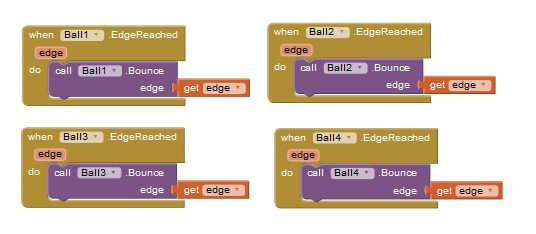
\includegraphics[width=10cm]{figures/apps/ai_collision_blocks}
\caption{Bloki odpowiedzialne za zdarzenia kolizji ze ścianą}
\end{figure}




\section{Zalety programowania wizualnego}

\section{Wady programowania wizualnego}

Przynajmniej na razie nie ma możliwości rozszerzenia App Inventora, więc jeżeli chciałbyś stworzyć coś lub skorzystać z czegoś, co nie jest wbudowane bezpośrednio w oferowaną platformę, jak np. grafika 3D, jesteś bez szans.

Implementacja App Inventora nie jest zoptymalizowana dla gier o wysokiej wydajności.
